\documentclass[10pt,a4paper,]{article}

\usepackage[english]{babel}
\usepackage[T1]{fontenc}
\usepackage[utf8]{inputenc}
\usepackage{graphicx}
\usepackage{url}
\usepackage{hyperref}
\usepackage{cite}


\pagestyle{headings}

\title{Teaching with Artificial Intelligence\thanks{Semestral project in the subject Engineering Methods, academic year 2020/21, leadership: Ing. Michal Hatala, PhD.}}

\author{Daniel Kajan\\
	{\small Slovak technical university in Bratislava}\\
	{\small Faculty of informatics and information technologies}\\
	{\small \texttt{...@stuba.sk}}
	}

\date{\small 30. October 2020}



\begin{document}

\maketitle

\begin{abstract}
The purpose of this work is to investigate the use of Artificial Intelligence in Education(AIED), its problems, its history and to speculate about its future. We view these issues as inherently social in nature. Technology is constantly evolving and shows no signs of stopping anytime soon. With this progress come advancements in artificial intelligence, which seeps into all other fields. So, we will take into account AI general terms, but also more specifically as it relates to education.
\end{abstract}



\section{Introduction}

Education has an \textbf{extremely high value} to us as a species. The older and wiser members teaching the
younger ones is nothing new and it has worked for millennia. 

However, with the \textbf{advent of technology} replacing the old with the newer and more modern, could this be the next thing to disappear in the passage of time? What would happen if we were to remove as much of the human factor as possible from the equation? And what if we were to replace it with Artificial Intelligence? Answers to these questions and some others is what we set out to find out.

We'll go over the \textbf{generalization of problems} relating to AIED in part \ref{general}. Some \textbf{potential applications} of AIED will be mentioned in part \ref{uses}. Part \ref{history} will relate to \textbf{the history of AI}, part \ref{future} addresses our \textbf{speculation about} where \textbf{the future} of the AIED research might take us. Finally, our thoughts will be compiled in part \ref{end}.

\section{General problems with AI and AIED} \label{general}

\paragraph{Social context.}

The priorities of education seem to be shifting from preparing students by giving them a vast array of knowledge in a field to teaching them how to become more adaptive in the workplace.\cite{Roll2016} We find this to be \textbf{a beneficial shift of direction}, because it doesn't just relate to the present, but makes the future the focal point.

Focusing on the future is exactly what we need to do with artificial intelligence. Many in the past have theorized about when AI will surpass us humans and so far didn't manage to get it right. Many still theorize on when this creation of ours will become a so-called \textbf{super-intelligence}, that we will no longer be able to control it and it may overthrow its creators some day. This is one of the \textbf{major problems with using AI in general}, but somewhat more so when it comes to education.

\paragraph{Sustainability and ethics.}

What we have to think about is that we also have to educate the AI itself. How do we do that, without risking a robot uprising? Do we limit ourselves based on the hardware we can use when creating AI? Do we try to encode it deep into the AI itself? Or will we just assume, that they will never surpass us, that we are unable to create something better than us? Though the last one may seem ridiculous, it is necessary to ask these questions.

One could argue that we seem to be nowhere near creating an AI good enough for it to even attempt hurting humanity. It certainly seems to be the case, but we wonder if we as humans are even capable of predicting which of the thousand small steps we're constantly taking will take us over the edge.

Even in our current situation, \textbf{AI assisted learning is catching up to the human tutoring variety.}\cite{VanLehn2011} And as this area will continue to improve, more and more voices will most likely arise about the dangers of AI and implementing it into education. Companies will have troubles marketing this to broader audiences.\cite{KRAFFT2020}

Other than politics and fields that directly deal with matters of survival like the medical field or military, the application of artificial intelligence in education is potentially \textbf{the scariest one.} There could come a point where we just have no idea what the AI is teaching students, because at that point it might be adapted on a \textbf{too large} of a scale.

And it is only after taking all of these inherent concerns and dangers into consideration, when we can focus on how exactly we can implement artificial intelligence into education.

\section{Uses of AI in Education} \label{uses}

The first option that we would like to take a look at is \textbf{Personalized Learning}. The idea of it is to personalize training materials on an individual basis. It attempts to identify the students strengths, weaknesses, needs, skills and interests and use them to create a better learning environment. Thanks to AI, things like adaptive user interfaces can be created\cite{Jiming2003}. Researchers have also used smart sensors and wearable devices for self-regulated learning\cite{Ciolacu2018}.

The second option we would like to present is one that aims to help teachers through the use of \textbf{AI to simplify administrative tasks}. It can be used in grading tests, assessing homework\cite{LLAMASNISTAL2013} and making responses to students more automatized\cite{Park2019}.

The third is using AI to reach a wider audience. \textbf{Presentation Translator} serves as a perfect example. It is a "free plugin for PowerPoint, which creates subtitles in real-time of what the teacher is saying, displaying them below the presentation. Using Azure Cognitive Services, AI-powered speech recognition and translation allows students to hear or read what is being said in their own native language."\cite{McNeill2018}

\section{A brief history of AI} \label{history}

\paragraph{Historical context.}

Even before the actual creation of any AI, many science fiction writers came up with different robots, golems and automatons in their works. There have also been some physical attempts at creating imitations of life. Mechanical animals and dolls based on clockwork mechanisms and the famous hoax called \textbf{The Turk} come to mind.\cite{Buchanan2005}

Artificial Intelligence more accurately dates back to the 1950's to \textbf{Alan Turing's} proposed solution to the question as to when we should classify a system as intelligent. More specifically we can attribute the beginning of this field to 1956 when \textbf{John McCarthy} coined the term 'artificial intelligence' at a conference at Dartmouth College, in Hanover, New Hampshire.\cite{Popenici2017}

\begin{figure}[h]
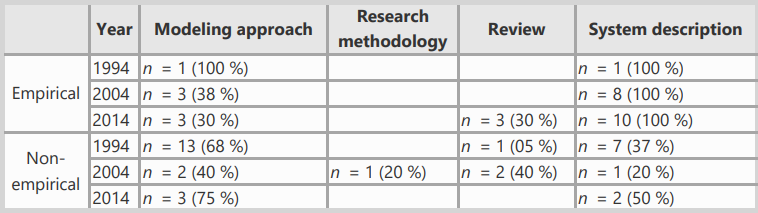
\includegraphics[width=\textwidth]{Kajan_MIP_tabulka.png}
\caption{A table showing the changing aims of AIED papers. \cite{Roll2016}}
\end{figure}

\begin{figure}[h]
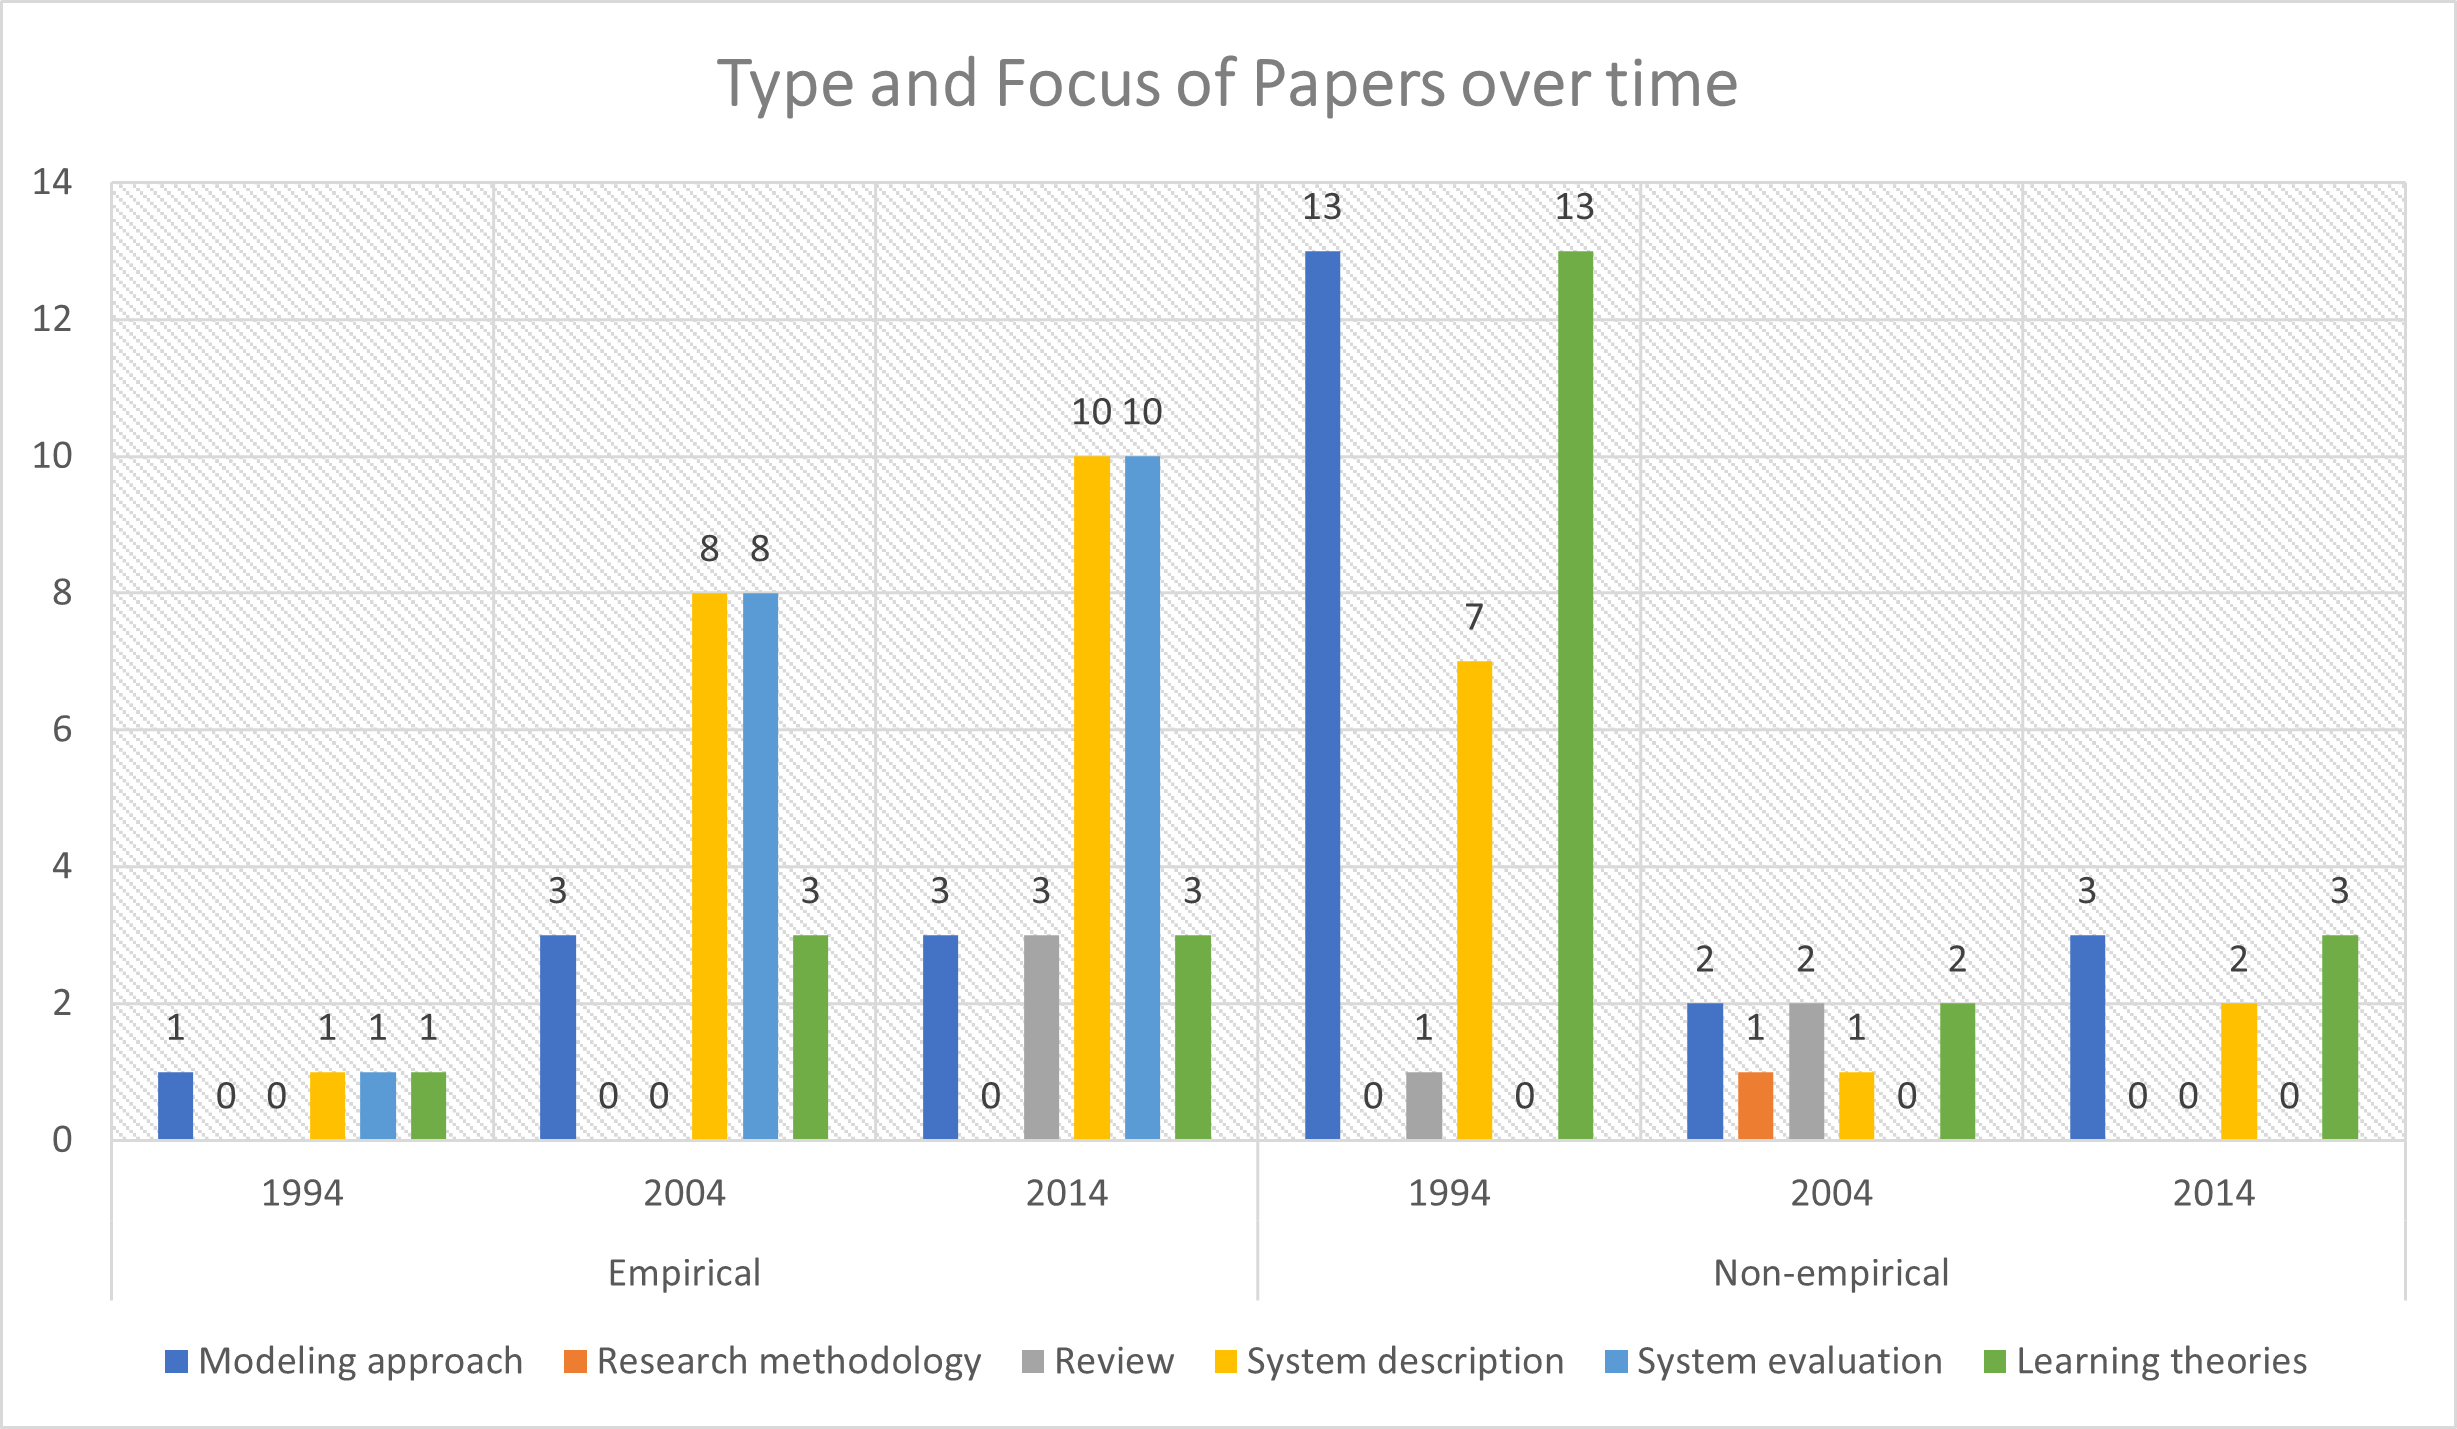
\includegraphics[width=\textwidth]{Kajan_MIP_diagram.png}
\caption{A diagram showing the changing aims of AIED papers. \cite{Roll2016}}
\end{figure}

\paragraph{Technology and people.}

\textbf{Marvin Minsky} is quoted at the time to have said that the problem of artificial intelligence will be substantially solved "within a generation". Early programs were greatly limited. New power was given to the programmers only after the creation of \textbf{Symbol manipulation languages and time sharing systems} in the 1950's and 1960's. The first really good program was \textbf{Arthur Samuel's} checker-playing program, which was actually able to improve through experience.\cite{Buchanan2005}

During its less than 70 year long history, this field has already experienced two major time periods without any substantial improvements to note. These are the years 1974-1980 and 1987-1993. A big break however, came in 1997, when \textbf{IBM's Deep Blue} became the first computer to beat a chess champion. A later accomplishment of this tech giant came in 2011 when \textbf{IBM's Watson} won Jeopardy! while playing against Brad Rutter and Ken Jennings.\cite{USA2016}

\section{The potential futures of AI} \label{future}

Something that we might look forward to within our lifetimes are fully autonomous vehicles and aircraft. Many cars now have driver assist features like self-parking and advance cruise controls. Some fully automated cars have been tested already, but this was usually in closed environments or under human supervision. All we can hope for now is for the law the catch up and brings us closer to a future, which seems just like science fiction right now.\cite{USA2016}

A great deal of progress has been made in what's known as \textbf{Narrow AI}. This type of AI only addresses specific tasks and is used only in the one scenario that it has been purpose-built for. \textbf{General AI} (also referred to as Artificial General Intelligence, or AGI) is a term used to describe a theoretical intelligence, which is as intelligent or more intelligent than a person in every cognitive task. The general consensus now is that this kind of AI will not be achieved for at least a few decades.\cite{USA2016}

We can only speculate when we'll get AI teachers into our schools. So far the steps of AIED seem to follow a path of improving the work that the flesh and blood counterparts do on the daily basis. This area doesn't even have any big inherent dangers within it, since an AI which just answers your emails doesn't need to be very complex and therefore that intelligent.

Looking a bit ahead we could see a future where an AI assistant could maybe just change up the teachers assignment a bit here and there to make it easier to understand for students who might be struggling in the teacher's subject. If we got to this point, than maybe we could expect an AI to tutor some of those who might need it. But these are just mere conjectures of the mind at this point. We just have to wait and see what the future holds.

\section{Conclusion} \label{end}

Overall, AI is as exciting as it is possibly dangerous. We are unable to predict when AI becomes truly dangerous to us, but one thing is clear. We have to be ready before it can happen. Though this very likely might miss all of us living today. Artificial Intelligence as a term has been with us now for 64 years and the plethora of assumptions regarding our doomsday at the hands of robots were very off.

In any case, losing sleep over this will do us no good. Those of us who aren't out there trying to create the next best AI should put our trust in people who are and in the institutions and government overlooking their work.

What we should be doing instead is to get excited at the prospect of new emerging technologies bringing us forward as a species. Drones, cars that drive themselves, algorithms which translate spoken language for us in real-time and through that bringing us together, smart homes, personal assistants and so much more.

The work of a teacher especially is one of the most taxing jobs out there. Why not let them have a little help when we can provide it? We will not get AGI teachers tomorrow, but we can make gradual changes that get us closer and closer to that reality everyday.

We should also note that just being around AI and having it available to them might entice students to pursue a career in this field, aiding research and our progress. The future has a lot in store for us. And it will be great to find out what exactly it is.

\bibliography{Kajan_zdroje}
\bibliographystyle{unsrt}
\end{document}
